\documentclass[apj]{aastex}
\shorttitle{Delay Time Distributions of SNe~Ia}
\shortauthors{Strolger et al.}

\usepackage{natbib}
\usepackage{nicefrac}
\usepackage{ulem}
\usepackage{xcolor}
\usepackage{amssymb,amsmath}
\bibliographystyle{apj}

\renewcommand{\deg}{^{\circ}}
\begin{document}
\title{The Empirical Delay Time Distributions of Type Ia Supernovae From Galaxy Star Formation Histories}
\author{L.-G.~Strolger, Pacifici, Rodney, et al.}

\begin{abstract}
blah, blah, blah \ldots
\end{abstract}

\section{introduction}

\section{Description of the Data}

\section{Delay Time Distributions from Star Formation Rate Densities}

\section{Delay Time Distributions from Star Formation Histories}
This is an evaluation of the maximum likelihood delay time distribution following the prescription of \cite{Maoz:2012a} but performed on the GOODS/CANDELS galaxies. In a given galaxy, the total expected rate of SNe~Ia per year will be:
\begin{equation}
R_i = \int_0^t \Psi(t') \ast \Phi(\tau)\,dt'
\end{equation}
\noindent where $\Psi(t)$ is the star formation history of the galaxy (mapped in forward time), and $\Phi(\tau)$ is the delay time distribution model, also forward in time. The product of the integrated rate and the control time, $t'_{c, i}$, which contains all the information on the temporal sampling and depth of the survey, 
\begin{equation}
m_i = R_i \times t'_{c, i}
\end{equation}
\noindent which is the expected number of SN Ia events from that galaxy over the duration of the survey. The probability distribution of observed events is likely Poisson, where of catching $n_i$ SNe~Ia from that galaxy when $m_i$ are expected is
\begin{equation}
P(n_i | m_i) = \frac{m_i^{n_i}e^{-m_i}}{n_i!}.
\end{equation}
The product of probabilities for all galaxies in the survey would then serve as the likelihood of a given delay-time distribution model. The log-likelihood, convenient for MCMCs, is then expressed by:
\begin{equation}
L = \prod _i^N P(n_i|M_i) \Rightarrow \ln L = -\sum^N m_i+\sum^N\ln\biggl(\frac{m_i^{n_i}}{n_i!}\biggr)
\end{equation}
\noindent in which the last term is zero for galaxies which do not host SNe~Ia during the survey.

Following \cite{Strolger:2010}, we can continue to test a robust delay-time model, capable of reproducing the theoretical distributions for SD and DD models at one extreme, and $\delta$-function delay times at the other. The unimodal, skew-normal $\Phi(\tau)$ function is defined as:

\begin{equation}
	\Phi(\tau)=\frac{1}{\omega\pi}\,\exp\biggl(\frac{-(\tau-\xi)^2}{2\omega^2}\biggr)\int_{-\infty}^{\alpha (\frac{\tau-\xi}{\omega})} \exp\biggl(\frac{-t'^2}{2}\biggr)\,dt',
\label{eqn:model}
\end{equation}

\noindent where location ($\xi$),\footnote{Different from the initial mass function, $\xi(M)$.} scale ($\omega^2$), and shape ($\alpha$) define the mode time ($\bar{\tau}$, as defined in the previous tests), variance ($\sigma^2$), skewness ($\gamma_1$), and kurtosis ($\gamma_2$) of the model function by,

\begin{eqnarray*}
 \bar{\tau}&=&\xi+\omega\delta\sqrt{\frac{2}{\pi}},\\
 \delta&=&\frac{\alpha}{\sqrt{1+\alpha^2}},\\
 \sigma^2&=&\omega^2\biggl(1-\frac{2\delta^2}{\pi}\biggr),\\
\gamma_1&=&\frac{1}{2}(4-\pi)\frac{(\delta\sqrt{2/\pi})^3}{(1-2\delta^2/\pi)^{3/2}},\\
\gamma_2&=&2(\pi-3)\frac{(\delta\sqrt{2/\pi})^4}{(1-2\delta^2/\pi)^{2}}.\\
\end{eqnarray*}

The model parameters, $\xi$, $\omega$, and $\alpha$ are explored in an Affine Invariant Markov-chain Monte Carlo using {\tt emcee.py} \citep{Foreman-Mackey:2013pd}. As for priors, we restrict the parameters to the space:

\begin{eqnarray*}
-15 <&  \xi &\le 15\\
0 <&\omega &\le 15\\
-15 <&  \alpha &\le 15\\
\end{eqnarray*}


\begin{figure}[t] %  figure placement: here, top, bottom, or page
   \centering
   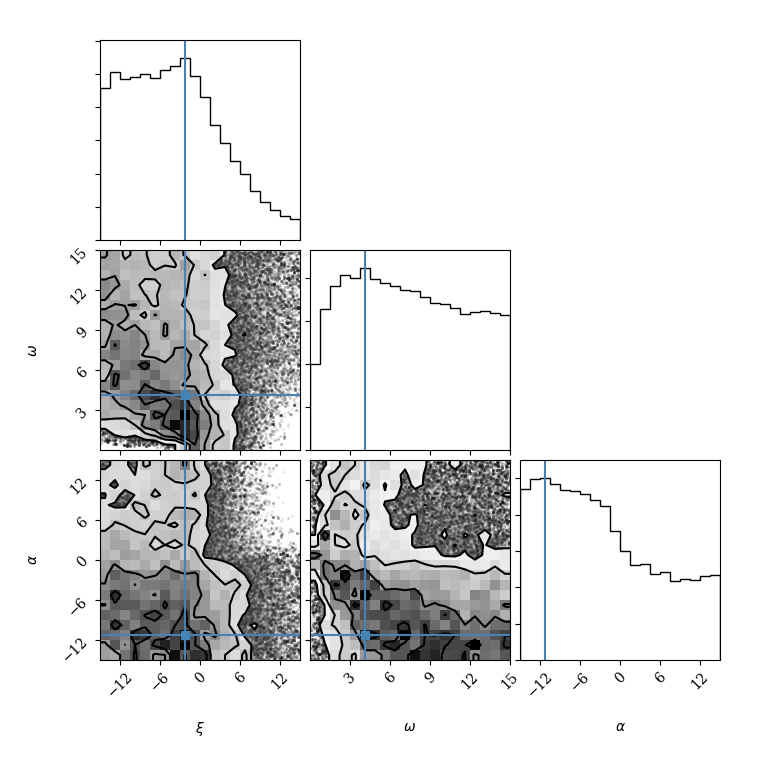
\includegraphics[width=4in]{Figure_1} 
   \caption{\footnotesize MCMC results on 147 galaxies in CANDELS, 49 of which are SN~Ia hosts. Plot generated using {\tt corner.py} \citep{Foreman-Mackey:2016ve}.}
   \label{fig:fg1}
\end{figure}
\begin{figure}[h] %  figure placement: here, top, bottom, or page
   \centering
   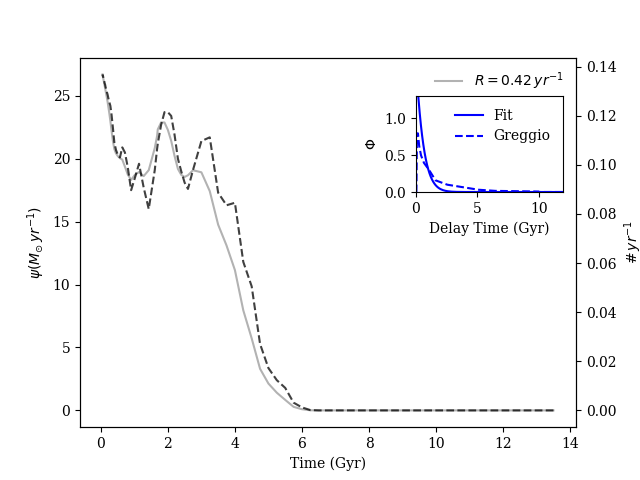
\includegraphics[width=4.5in]{Figure_2} 
   \caption{\footnotesize Example of best-fit delay-time distribution (inset) on the SFH of a sample host galaxy. }
   \label{fig:fg2}
\end{figure}

\section{discusssion}

\bibliography{strolger}{}

\end{document}